\documentclass{report}

\usepackage{attrib}
\usepackage{hyperref}
\usepackage[pdftex]{graphicx}

\begin{document}

\title{Are You Out-ethics on Shopping?}
\author{Terrence Monroe Brannon \\
thequietcenter@gmail.com }
\maketitle

\tableofcontents

\chapter{Introduction}

\begin{quotation}
THE DYNAMIC PRINCIPLE OF EXISTENCE IS SURVIVE! ... one of the best guarantees of survival is abundance.
\attrib{\emph{Science of Survival}, L. Ron Hubbard}
\end{quotation}

\begin{quotation}
The highest ethic level would be long-term survival concepts with minimal destruction, along any of the dynamics.
\attrib{\emph{Scientology Tech Dictionary}, Definition of Ethics, L. Ron Hubbard}
\end{quotation}


\begin{quotation}
You have to shop in order to survive
\attrib{Andy T. Hansen}
\end{quotation}

\section{Shopping is a survival concept}

Our introductory quotes imply that shopping is central to survival, yet, the topic of shopping is at first glance insultingly obvious --- almost like trying to teach someone to breathe. \emph{``Who doesn't know how to shop? I've done it every day for decades!''} The common mode of shopping is so widely accepted that open-minded, objective, quantitative inspection of it will almost certainly lead to outrage and criticism. Be that as it may, the purpose of this article is to compare various shopping approaches in terms of ethics.

There are countless viewpoints on shopping and its relation to survival. Many of these viewpoints shun shopping and emphasize other approaches to survival. Freganism, for instance, uses any means possible to obtain living essentials without paying. They will eat food from tables after people have left them. They will search through garbage bins. They will sleep wherever they are offered residence. They will barter instead of paying money. Because fregans survive and do not shop, there is no question that it is possible to survive without shopping.

However a great number of $1^{st}$ dynamics do rely on shopping for survival. And many of those $1^{st}$ dynamics would agree with the quotations that opened this section. Those quotations, logically connected, lead to this conclusion:

\begin{quote}
Ethical shopping requires and should produce monetary income that is stable and abundant over multiple dynamics.
\end{quote}

With this expectation of ethical shopping, let us see just how ethical various modes of shopping are.

\section{Definitions}

\subsection{Sample hybrid dynamic}
Per the definition of ethics, we still be studying shopping stability across dynamics 1-4. I coin the term \emph{sample hybrid dynamic} for this purpose. Our sample hybrid dynamic starts with a $1^{st}$ dynamic named Jill. On her 2d, Jill reproduces with Jack 5 times, creating 5 children. These 5 children follow suit and also create 5 offspring, leading to 25 grandchildren. These 25 grandchildren all have 5 distinct members in their 3d leading to 125 people with whom they collectively have A.R.C.  

\begin{figure}[h]
\centering
	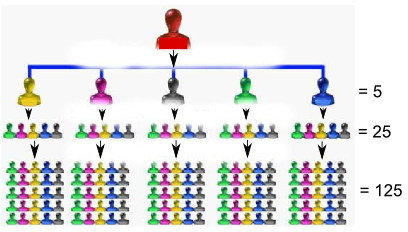
\includegraphics[width=2in]{sample-hybrid.png}
	\caption{sample hybrid dynamic connecting 1d, 2d, 2d' and 3d}
	\label{fig:sampleHybridDynamicOf125Terminals}
\end{figure}

\subsection{ARC Span}\label{def:arc_span}
ARC Span is a numerical sum indicating the people with whom you directly or indirectly have high levels of affinity with. This is an expansion upon the LRH concept of ARC, which only took into account direct affinity. Let's look at an example. Let's say that Jill has good ARC with her husband. And let's say that the husband has 2 people he plays cards with every Wednesday. This means that Jill's ARC Span is 1 + 2, 1 for direct ARC with her husband and 2 for indirect ARC with her husband's card playing buddies. The sample hybrid dynamic shows Jill to have an ARC Span of 1 + 5 + 25 + 125 or 156.

\subsection{Superlinear}
Let's define superlinear by contrast with the related terms linear and sublinear. A linear function shows constant rate of change for increasing values of x. For instance the linear function y = 3x has a constant rate of change of 3. A sublinear function shows decreasing rate of change for increasing values of x. A superlinear function shows increasing rate of change for increasing values of x. 

\begin{figure}[h]
\centering
	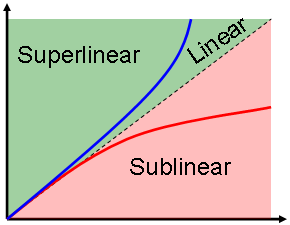
\includegraphics[width=2in]{superlinear.png}
	\caption{superlinear, linear, and sublinear graphs}
\end{figure}

\subsection{Shopping} the exchange of money for goods and services.

\subsection{Shopping power} money. The ability to buy.  

\subsection{Ethical shopping}
shopping that yields superlinear long-term shopping power as a function of the number of dynamics. In other words, as the number of people in Jill's sample hybrid dynamic increases from 1 to 2 to 5 to 25 to 125, we would like to see a superlinear increase in her shopping power. This is ideal for Jill. There may or may not be such a shopping model, but it is clearly the most ideal thing she could hope for.

\subsection{Second dynamic}
I define second dynamic as ``sex and the rearing of children \emph{who eventually rear their elders}.'' This is an important extension of LRH's original definition. While it makes sense for the elders to nurture and raise young children, at a certain point, the children will be healthier and have more earning power than their elders and the responsibility falls to them to insure the welfare of the ones who once cared for them.

\subsection{Residual}\label{def:residual}
something that provides output without additional input. For instance, if an insurance salesman writes a car insurance policy for a customer, the salesman earns money each month that the insurance policy is paid --- he worked one time to produce income for an entire year. In contrast, a career as a Scientology auditor is not residual. You only earn income when you are sitting in the chair auditing a terminal.

\section{Expectations}

Per the definitions above, we are trying to find a shopping model that yields superlinear shopping power as a function of ARC Span. I.e., as her sample hybrid dynamic grows, her shopping power should stabilize, strengthen and increase.

Synergy is a well-known effect.The power of groups can greatly amplify individual efforts in fields as diverse as ecstatic religious experience and walking across a bridge. Similar synergy is expected from an ethical shopping model.

\chapter{Examination}
\section{Traditional shopping}

In the traditional shopping model, one shops for his goods or services, pays full price for them, and then leaves with his goods and a receipt. Normal enough you might think. But how ethical is this mode of shopping? Let's step through our sample hydrid dynamic and see. We will make the assumption that all people have \$4000 monthly income and spend \$1500 a month on various necessities.

\subsection{Jill as 1d}
Jill shops traditionally and simply gains good and services for her money. With an income of \$4000 and expenditures of \$1500, she ends up with \$2500 in shopping power.

\subsubsection{Jill as 2d}
\label{2dtraditional}
Jill marries Jack and their money doubles and they continue to shop the same way. They now have an income of \$8000 and we would presume that the necessities only increase by 50\% since some of the necessity costs are now shared. So when Jill extends from 1d to 2d, she has \$8000 income and \$2250 in expenditures for a net shopping power of \$5750. This is slightly superlinear. A perfectly linear gain would have been \$5000. So we see a bit of improvment in shopping power by marriage.

\subsection{Jill's 2d rears 5 children}
\label{2d'traditional}
    5 offspring are produced by Jack and Jill. While rearing these children their shopping power drops because of increased necessities. Eventually all 5 children grow up and are able to earn money for themselves. Presuming no retirement for Jack and Jill, their shopping power returns to \$5750. And even though the children are concerned with their parents, they have to focus on their own lives and finances. So they dont contribute anything to Jack or Jill. So the production of 5 children represented a drop in shopping power for 18 years and a return to the baseline value of \$5750. To have 5 more offspring and yet have the same buying power as 2 people is sharply sublinear.

\subsection{Jill's 5 children each produce and rear 5 offspring}
    The 5 offspring, then each create 5 children, who continue the trend of focusing on their own needs. This again leads to no gains for Jack and Jill. So we see that as the 2d expands to 2d', the shopping power of Jack and Jill remains constant at \$5750 - assuming that Jack and Jill remain healthy and capable of earning an income.

\subsection{Jill's 25 grandchildren form various 3d groups}

The sublinear buying power trend increases as the 2nd dynamic branches out into the 3rd dynamic. Now we have 125 people who all contribute nothing to Jill's shopping power.

\subsection{Reflection}

Jill's shopping power levelled off while ARC Span continued to increase. This is contra-survial. How ethical is it for a group of 125 people to be no more powerful in their shopping power than an isolated first dynamic? How ethical was it for Jack and Jill to reduce their shopping power for 18 years or more with no clear return on their investment? Recalling that shopping power is directly related to survival, we really have to call the traditional shopping model into question. The graph below shows the relation between shopping power and dynamics growth in this model of shopping.

\begin{figure}[h]
\centering
	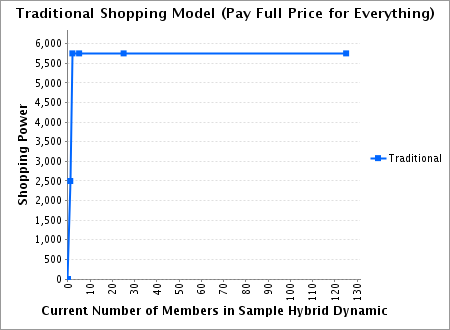
\includegraphics[width=3in]{shopping-traditional.png}
	\caption{The traditional model of shopping does not translate ARC Span into Shopping Power}
\end{figure}


\section{Coupon discount programs}

Let's step through our sample hybrid dynamic and see how Jill and her sample hybrid dynamic fare when adding coupons to their shopping. Let's assume that they can effect a 20\% reduction in costs via coupons. 

\subsection{Jill as 1d}
\label{1dcoupon}
As a solo 1d, Jill has \$4000 as income. Her \$1500 in expenditures has been reduced to \$1200 because of the savings from using coupons. Therefore, instead of only having \$2500 dollars after shopping, she has \$2800.

\subsection{Jill forms a 2d}
In \ref{2dtraditional} we examined Jill's 2d shopping in the traditional fashion. Let's see what happens here. 

The first thing that happens is that Jill's income doubles - instead of \$4000 in income, she now has \$8000 to play with. We will also carry over the assumption that the expenditures of a married couple are \$2250.\footnote{compared with \$1500 for Jill as solo 1d} Now, applying our 20\% coupon discount to the expenditures reduces them to \$1800. 

So, as 2d, Jill has \$6200 in shopping power after her monthly cycle of receiving money and paying for necessities for herself and her husband. This is a gain over the \$5750 we saw in  \ref{2d'traditional}.

\subsection{Jill's 2d rears 5 children}

    The 5 offspring are produced who then grow up and pursue couponing as well. Their personal money increases but there is no compulsion to help Jill and Jack with their shopping necessities. So for the remaining dynamics, we see the same trend in couponing as we did in the traditional shopping model - increasing ARC Span but no certain increase in shopping power  for Jack or Jill.

\begin{figure}[h]
\centering
	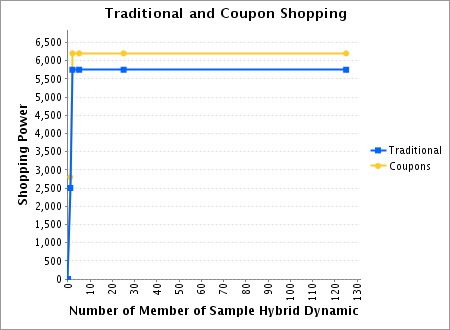
\includegraphics[width=3in]{shopping-coupon.png}
	\caption{Ethical comparison of traditional and coupon shopping}
\end{figure}
  
\section{Simple cashback}

From a mathematical perspective, simple cashback and coupon savings are exactly the same. If you have \$100 in your bank account and you want to buy a book that costs \$10, then getting a 25\% discount on the book means it costs you \$7.50 and you have \$92.50 in the bank after buying it. Likewise, if you paid full price for the book and received 25\% cashback, you would end up with \$92.50 in the bank after paying full price and then getting cashback, i.e. \$100 - \$10.00 + \$2.50 = \$92.50.

But cashback has some interesting \emph{residual} (see \ref{def:residual}) aspects, because the cashback can be automatically disbursed to a chain of people. In other words, we were looking for a financial analogue to the chain of ARC we defined using the term ``ARC Span'' (\ref{def:arc_span}) and we may have found it.

Having \href{http://www.CashbackPrograms.info/report}{surveyed a large of number of cashback programs}, I found that the cashback disbursement chain varies from 0 to infinity. For instance some cashback programs (e.g. credit card rewards programs) only allow you to get personal cashback. Other programs allow you to get cashback from your direct referrals but not indirects. Others provide cashback on 2 levels of referral. Only 3 programs provide deeper cashback networking. They will be discussed in the following sections.

For now, let's look at how shallow cashback systems affect shopping power. We will take the 20\% coupon savings we studied in the last section and distribute the same percentage as cashback savings along a chain. Let's assume that for each purchase made, 20\% cashback is disbursed as follows:

\begin{enumerate}
\item    the purchaser gets 15\% cashback
\item    your sponsor gets 2.5\% cashback
\item    your sponsor's sponsor get 2.5\% cashback.
\end{enumerate}

Now we will examine how ethical simple cashback shopping is:

\subsection{Jill as 1d}

We start with the same income for Jill --- \$4000. Her monthly expenditures are \$1500 and she gets 15\% cashback, or \$225. So her net shopping power is \$4000 - \$1500 + \$225 or \$2725. For Jill's purchases, it is also the case that 2.5\% cashback goes to her immediate and indirect sponsor, but they are irrelevant in terms of us studying Jill's shopping power.

Compared to coupon shopping (\ref{1dcoupon}), simple cashback seems less ethical. With coupons, Jill got the whole 20\% savings for herself. With simple cashback, she only got 15\%. But let's withold judgement until we've examined this program fully.

\subsection{Jill forms 2d with Jack}

    Jill marries Jack and also sponsors Jack into the cashback program. What this means is that Jack's purchases yield 15\% cashback for himself 2.5\% for his sponsor (Jill). Collectively, this yields 17.5\% in cashback benefits for them, presuming Jack does all the purchasing. Their income remains \$8000. They spend \$2250 in bills and get 17.5\% cashback on those expenditures, or \$393.50, so their net shopping power is \$8000 - \$2250 + \$393.50 or \$6143.50.

\subsection{Jill's 2d produces 5 offspring}

    5 offspring are produced. Now, each of the 5 offspring are sponsored into the cashback program by Jack. This means that when the offspring spend money, the offspring get 15\% back, Jack gets 2.5\% back, and Jill also gets 2.5\% back. Since Jack and Jill operate as a single married entity, we can calculate the cashback on their offspring's purchases as 5\%. The innate urge to survive compels the offspring to save money when they can and so they get cashback whenever they can. However, in contrast to couponing, there is no need to manually send their parents money. Instead, cashback flows automatically from offspring to parents. So, each married family has \$8000 in income. In the interest of helping their elders they only take out one cashback sponsorship per family. So they only get 15\% cashback instead of one spouse getting 15\% and the other getting 2.5\%. At this rate, they spend \$2250 in bills and get \$337.50 in cashback. So each family has a net shopping power of \$8000 - \$2250 + \$337.50 or \$6087.50. 
  
But the interesting thing is that Jack and Jill also get some cashback while their offspring do. They get 5\% of \$2250, or \$112.50. And multiplying this by 5 offspring means they get \$562.50 in residual earnings from their childrens shopping. This increases their net shopping power from \$6143.50 to \$6706.
    
\subsection{Jill's 5 offspring each produce 5 offspring} 

    The 5 offspring each bear 5 children. This is 25 children who eventually grow up sponsored in the same cashback program. So, focusing on Jack and Jill's earnings, they will get 2.5\% of every \$2250 spent by their 25 grandchildren or \$1406.25. Jack and Jill's grandchildren increase their net shopping power from \$6706 to \$8112.50.

\subsection{Jill's 25 grandchildren form various 3d groups}

    When the 25 grandchildren branch out into their various 3d, there is no cashback for Jack and JIll because this simple cashback network is only 2 levels deep. So their shopping power remains at \$8112.50.

So the simple cashback network offers residual income. Jill, the root of our sample hybrid dynamic, shows increased shopping power for the early growth of her sample hybrid dynamic. However, ethics requires stability along all dynamics and the simple cashback network does not provide this from the grandchildren's 3rd dynamic because the referral network is not deep enough. 

\begin{figure}[h]
\centering
	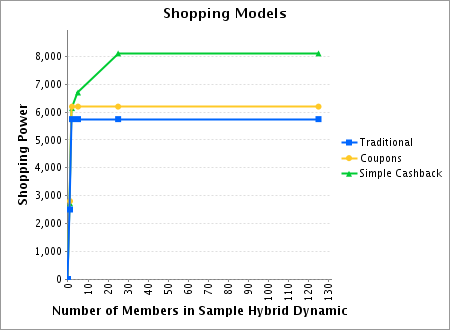
\includegraphics[width=3in]{shopping-simple-cashback.png}
	\caption{Ethical analysis of simple cashback shopping. It's certainly more ethical, but can we do better?}
\end{figure}

\section{Deeply networked cashback}

Let's take a moment to review what we have seen so far.We first saw that the conventional method of shopping is ethical suicide. It offers no possibilities for improving shopping power as the sample hybrid dynamic forms. With simple cashback, we saw significant advantages over the previous methods of shopping. 
We saw Jill earn residual income. She simply sponsored members of her ARC Span into the cashback program one time and she earned income on their shopping month after month.

However, we also noticed that as our sample hybrid dynamic grew, the earnings did not continue to grow. Simple cashback shopping is definitely more ethical than the other models we have seen so far. But ethics demands stable abundance along all dynamics for our shopping. Let's move on to models of cashback shopping which provide for deeper cashback compensation. To study deeply networked cashback we will look at \href{http://j.mp/cbk-beesavy}{one well-designed deeply networked cashback system --- BeeSavy} . A youtube video entitled ``BeeSavy Tutorial - What is Referral Cash Back?'' gives a demonstration of the Beesavy compensation. The chart below summarizes the video. 

\begin{figure}[h]
\centering
	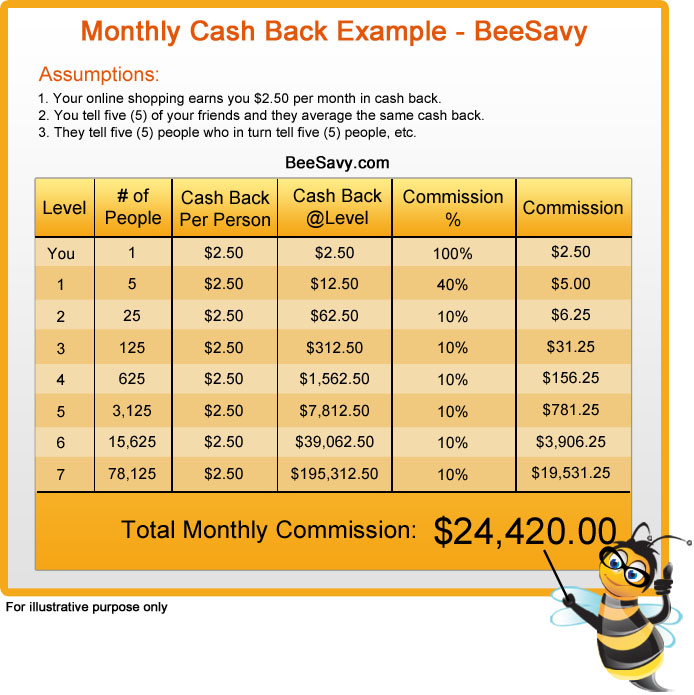
\includegraphics[width=3in]{beesavy-table.png}
	\caption{BeeSavy compensation plan}
\end{figure}

 

In our example, the total cashback was 20\%. In order to ration this across 8 levels, we will provide the following cashback percentages per level:

\begin{enumerate}
\item   10\%
\item 4\%
\item  1\% for the remaining 6 levels
\end{enumerate}	

Now that we see how much cashback Jill will be receiving from various levels of her sample hybrid dynamic, let's step through her dynamics one by one to see just how ethical deeply networked cashback is.

\subsection{Jill as 1d}

    So Jill has \$4000 income as normal. She spends the full amount of \$1500 and she gets 10\% cashback, or \$150. So her net shopping power is \$4000 - \$1500 + \$150 or \$2650. 
    
At first glance, we see the worst 1d results we have seen yet outside of traditional shopping. Simple cashback offered the 1d 15\% cashback and couponing 20\%. We only see 10\% here. But again, let's step through all dynamics before drawing a conclusion.
    
\subsection{Jill shacks up with Jack, forming a 2d}  

    Jill marries Jack and also sponsors Jack into the cashback program. She lets Jack do all the shopping so that their net cashback increases to 14\%. They have \$8000 in income. They spend the full \$2250 in bills and they get 14\% of those expenditures back as cashback or \$315. So their net shopping power is \$8000 - \$2250 + \$315 or \$6065.

\subsection{Jill reproduces 5 times}
  
Jill produces 5 offspring. Once they are old enough to support themselves, they are sponsored into the cashback program by Jack. This means that when the offspring spend money, they get 10\% back and Jack and Jill get 5\% back. The innate urge to survive compels the offspring to save money so they get cashback whenever they can. However, in contrast to couponing, there is no need to manually send their parents a portion of their savings. Instead, cashback flows automatically from offspring to parents. 

Each married family has \$8000 in income. In the interest of helping their elders they only take out one sponsorship per family. So they only get 10\% cashback instead of one spouse getting 10\% and the other getting 4\%. At this rate, they spend \$2250 in bills and get \$225 in cashback. So each family has a net shopping power of \$8000 - \$2250 + \$225. 

But the interesting thing is that Jack and Jill also get some cashback while their offspring do. They get 5\% of \$2250, or \$112.50. And multiplying this by 5 offspring means they get \$562.50 in residual earnings from their childrens shopping. This increases their net shopping power from \$6143.50 to \$6706. 

\subsection{Jill's children produce grandchildren}

    The 5 offspring each bear 5 children. This is 25 children who eventually grow up, sponsored in the same cashback program. So, focusing on Jack and Jill's earnings, they will get 1\% of every \$2250 spent by 25 children or \$22.50 $\times$ 25 = \$562.50. The additional \$562.50 raises the income of Jill from \$6706 to \$7268.50.

\subsection{Jill's granchildren form 3d relationships}

    When the 25 grandchildren branch out into their various 3d, Jack and Jill receive 1\% of their shopping as well, so we have \$22.50 $\times$ 125 or \$2812.50. This increases their shopping power to \$10317.50.
    
\subsection{Reflections: Theta-level shopping}

With deeply networked cashback, we begin to see the stirrings of ``theta-level shopping.'' What on earth is theta-level shopping? Well, it's when theta simultaneously operates multiple bodies via shopping. With all of the former shopping methods, one would think there was a one-to-one correspondence between a spiritual being and a single body. However, we know that theta can perform ethically on multiple bodies simultaneously: 


\begin{quotation}
One theta body can take care of several individuals and ordinarily does.
\attrib{\emph{Time Track of Theta}, LRH}
\end{quotation}

It is only with deeply networked cashback that it appears that theta is operating multiple dynamics in the interest of the $1^{st}$ dynamic. In all other cases, there was too little monetary cooperation amongst the dynamics to think that a single thetan was truly operating from an ethical standpoint across multiple dynamics.

\begin{figure}[h]
\centering
	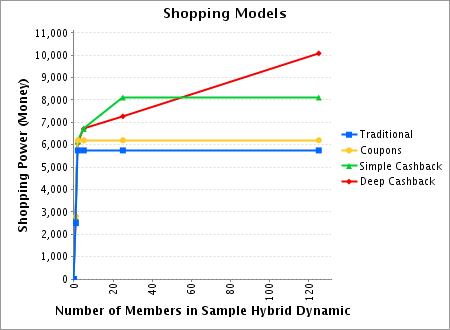
\includegraphics[width=3in]{shopping-deep-cashback.png}
	\caption{Ethical comparison of deeply networked cashback with previous models}
\end{figure}

\subsection{Reflections: Drawbacks of This Approach}

Deeply networked cashback is clearly more ethical than common shopping, coupon shopping and simple cashback shopping. We see residual gains that strengthen and increase through the entire depth of our sample hybrid dynamic.

However, as ethical as deeply networked cashback is, can we find some flaws? There are certainly a few:

\subsubsection{Online shopping only?}
BeeSavy is an excellent system, but it only offers online shopping. What this means is that you must opt for contra-survival shopping methods for your in-person shopping. Depending on your shopping tendencies, this will negatively impact the ethics of your shopping by a marginal or significant degree.

\subsubsection{8 levels is not infinite levels}
While 8 levels of cashback is probably enough to sustain the average first dynamic in our sample hybrid, it is a mathematical fact that 8 levels of cashback is not the same as infinite levels of cashback, or even 9 levels of cashback. Also ``enough to sustain'' is not the proper way to think about survival. From our introduction, we seek superlinear abundance. Thus, we seek to milk all of our connections along all dynamics to insure maximum survival. A system which makes this possible is ideal.

However, such a system has to ration the cashback in a vastly different way than the deeply networked model. Dividing the cashback along an infinite referral chain would lead to near-zero cashback for all members of the chain \footnote{E.g. rationing 20\% cashback along 100 levels would lead to a laughable 0.2\% per level}. The physical analogy of this problem would be trying to communicate to someone in another city by yelling - your voice would drop off in volume. To solve the problem of communicating, you need to package up the communication in electronic bundles and shuttle them along. The problem of registering cashback along infinitely long referral chains has a similar solution: an ``accumulative register'' of cashback shopping. In this way, local accumulations stay local, but are accounted for globally and infinitely.

\subsubsection{Charitable causes need our support}

Shouldn't the cashback company automatically disburse some of the cashback to worthy causes in the 4d, such as medical, environmental, and hunger funds? BeeSavy, our deeply networked model system, does not fund any such charitable effort.


\subsubsection{Sample hybrids operate in isolated, non-cooperative fashion}

Let's start this section by recalling how the universe works: shared realities will eventually intersect:

\begin{quotation}
Universe 1:

That universe, which you create for yourself. This is the universe, in which you can create for yourself spaces, planets, times, beings, ghosts, walls, barriers, energies, people, animals and plants along all impulses of exis�tence, where these creations are only perceivable for your self, and are only �there� for you. You are the one deter�mining the natural laws in your universe. You decide if there is gravitation, whether the clocks run backwards, or if objects move or are stationary.

Universe 2:

That universe, which every other SB creates for itself, as every other SB also possesses the ability to create its own personal universe with its own laws, sequences and func�tions inside his creations. It does not matter how big it is or if there are few or many things created. It can still be a closed system.

Universe 3:

The sum of illusions from Universe 1 and Universe 2 which has been agreed upon by all spiritual beings � the physical universe.

The �powerful� physical universe consists basically of nothing more than the co-created intersection of the dif�ferent individual universes. 
\attrib{\emph{Spiritologie}, Andreas Buttler}
\end{quotation}

Now, we have seen the success of Jill when using deeply networked cashback shopping over the sample hybrid dynamic. It is reasonable to presume the success of Jill can be duplicated by other $1^{st}$ dynamics. And per the quote above, a complete cashback system should allow people with similar universes to interact and help each other. But BeeSavy (and similar deeply networked systems) only allow for gains on one's personal ARC Span. 

In contrast, the infinitely networked cashback system allows for monetary cooperation between personal ARC spans residing in the same nation and continent.

\chapter{Conclusion}

In this article we have turned our attention to an overlooked part of daily life. Shopping is a survival process, but rarely seen that way. \footnote{Sex, eating and sleep are the most obvious ones.} Yet most people shop in order to survive. \footnote{Some do not, but those living at the highest survival levels do.} Traditional shopping is an out-ethics implant. The universal solvent is communication. It creates A.R.C. and A.R.C. leads to a network of A.R.C. Span. Using this A.R.C. to create permanent, infinite chains of cashback is a solution to stability on all dynamics for the the survival act of shopping.

The advantages of such a cashback network with no limits are not theoretical, but in fact actual. The system is showing many years of success and growth on all dynamics even beyond 1-4. Because a fraction of every cashback transaction is devoted to medical, education, or environmental causes, this program even addresses dynamics 5 and 6! Will all of your attention units be focused on the shopping of a single 1d, or will you shop in an ethical manner, promoting optimal survival along all dynamics?

\end{document}
